\documentclass[10pt,aspectratio=169,t]{beamer}

\usepackage[width=1600,height=900]{beamer-reveal}
\usepackage{fontspec}
\usepackage{unicode-math}
\usepackage{tikz}
\usepackage{booktabs}
\usepackage{array}
\usepackage{graphicx}
\usepackage{xcolor}
\usetikzlibrary{arrows.meta,positioning,fit,calc}

\setsansfont{TeX Gyre Heros}
\setmainfont{TeX Gyre Termes}
\setmathfont{TeX Gyre Termes Math}

\definecolor{iithblue}{HTML}{002147}
\definecolor{beamergrey}{HTML}{F2F5FA}
\definecolor{muted}{HTML}{4B5563}
\definecolor{accentgreen}{HTML}{006B5F}
\definecolor{accentred}{HTML}{8B0000}
\definecolor{linegrey}{HTML}{A9B4C5}

\setbeamertemplate{navigation symbols}{}
\setbeamercolor{normal text}{fg=black,bg=white}
\setbeamercolor{frametitle}{fg=iithblue,bg=beamergrey}
\setbeamerfont{frametitle}{series=\bfseries,size=\Large}
\setbeamertemplate{frametitle}{%
  \nointerlineskip
  \begin{beamercolorbox}[wd=\paperwidth,ht=0.82cm,dp=0.18cm,leftskip=0.45cm]{frametitle}
    \rule[-0.18cm]{0.08cm}{0.86cm}\hspace{0.18cm}\insertframetitle
  \end{beamercolorbox}
  \vspace{0.18cm}
}
\setbeamertemplate{footline}{%
  \leavevmode%
  \hbox{%
  \begin{beamercolorbox}[wd=.72\paperwidth,ht=2.2ex,dp=1ex,leftskip=0.45cm]{author in head/foot}%
    \scriptsize Traffic Interaction Authenticity \;|\; Waymax-backed counterfactual simulation
  \end{beamercolorbox}%
  \begin{beamercolorbox}[wd=.28\paperwidth,ht=2.2ex,dp=1ex,rightskip=0.45cm plus1fil]{date in head/foot}%
    \hfill\scriptsize \insertframenumber/\inserttotalframenumber
  \end{beamercolorbox}}%
}

\newcommand{\tightitem}{\setlength\itemsep{0.35em}}
\newcommand{\claimbox}[2]{%
  \begin{tikzpicture}
    \node[draw=linegrey, rounded corners=1.5pt, fill=white, inner sep=7pt, text width=0.91\linewidth, align=left] {\textbf{\color{iithblue}#1}\par\vspace{0.18cm}{#2}};
  \end{tikzpicture}%
}
\newcommand{\phasebox}[3]{%
  \begin{tikzpicture}
    \node[draw=linegrey, rounded corners=1.5pt, fill=white, inner sep=6pt, text width=0.92\linewidth, align=left] {
      {\scriptsize\bfseries\color{iithblue}#1}\par\vspace{0.05cm}
      {\bfseries #2}\par\vspace{0.05cm}{\scriptsize #3}
    };
  \end{tikzpicture}%
}

\title{Traffic Interaction Authenticity}
\subtitle{Counterfactual Evaluation and Adaptation of Learned Multi-Agent Traffic Simulators}
\author{Achyut Morang}
\institute{M.Tech Smart Mobility, IIT Hyderabad}
\date{}

\begin{document}

\begin{frame}[titleslide]
  \vspace{0.25cm}
  \begin{center}
    {\scriptsize\bfseries\color{iithblue}TENTATIVE THESIS DECK \;|\; SMART / CAT-K \;|\; WOMD / WOSAC / WAYMAX}\par
    \vspace{0.65cm}
    {\fontsize{34}{38}\selectfont\bfseries\color{iithblue}Traffic Interaction Authenticity}\par
    \vspace{0.35cm}
    {\large Counterfactual Evaluation and Adaptation of Learned Multi-Agent Traffic Simulators}\par
    \vspace{0.25cm}
    {\normalsize Achyut Morang \;|\; M.Tech Smart Mobility, IIT Hyderabad}\par
  \end{center}
  \vspace{0.45cm}
  \claimbox{Central claim}{A simulator can look realistic under ordinary closed-loop evaluation and still respond poorly to localized interventions. The object $p_\theta(\tau_{1:N}\mid H,M)$ is not the same as $p_\theta(\tau_{-j}\mid H,M,\operatorname{do}(\tau_j=\tilde\tau_j))$.}
\end{frame}

\begin{frame}{Story in One Slide}
  \begin{columns}[T,totalwidth=\textwidth]
    \begin{column}{0.32\textwidth}
      \claimbox{Problem}{WOSAC-style realism asks whether generated traffic looks plausible under logged initial conditions.}
    \end{column}
    \begin{column}{0.32\textwidth}
      \claimbox{Gap}{It does not directly ask whether nearby agents respond plausibly after a localized $\operatorname{do}()$ intervention.}
    \end{column}
    \begin{column}{0.32\textwidth}
      \claimbox{Evidence}{BC and CLSFT/CAT-K-style checkpoints can disagree between ordinary validation and counterfactual stress tests.}
    \end{column}
  \end{columns}
  \vspace{0.35cm}
  \begin{columns}[T,totalwidth=\textwidth]
    \begin{column}{0.32\textwidth}
      \claimbox{Substrate}{Waymax provides a reproducible branch environment for normal, forced, and placebo rollouts.}
    \end{column}
    \begin{column}{0.32\textwidth}
      \claimbox{Method}{Define Traffic Interaction Authenticity, validate structural critics, then consider conservative CIFT-CC adaptation.}
    \end{column}
    \begin{column}{0.32\textwidth}
      \claimbox{Ask}{Feedback is needed on framing, evidence gates, and the adaptation path.}
    \end{column}
  \end{columns}
\end{frame}

\begin{frame}{Problem Formulation}
  \large
  Ordinary sim-agent evaluation samples a future rollout:
  \[
    \hat\tau_{1:N} \sim p_\theta(\tau_{1:N}\mid H,M).
  \]
  The counterfactual diagnostic instead asks for responder behavior after one actor is externally changed:
  \[
    \hat\tau_{-j} \sim p_\theta(\tau_{-j}\mid H,M,\operatorname{do}(\tau_j=\tilde\tau_j)).
  \]
  \vspace{0.20cm}
  \claimbox{Key distinction}{The first asks whether generated traffic resembles logged traffic. The second asks whether generated traffic remains physically valid, map-valid, selectively responsive, and non-overreactive after a localized intervention.}
\end{frame}

\begin{frame}{SMART/CAT-K as the Baseline Substrate}
  \begin{columns}[T,totalwidth=\textwidth]
    \begin{column}{0.48\textwidth}
      \begin{itemize}\tightitem
        \item Road vectors become map tokens.
        \item Agent trajectories become motion tokens.
        \item RoadNet encodes map context.
        \item MotionNet predicts future tokens autoregressively.
        \item CLSFT/CAT-K-style post-training improves closed-loop behavior.
      \end{itemize}
      \vspace{0.2cm}
      \[
        p_\theta(z_{1:T}\mid H,M)=\prod_{t=1}^{T}p_\theta(z_t\mid z_{<t},H,M).
      \]
    \end{column}
    \begin{column}{0.48\textwidth}
      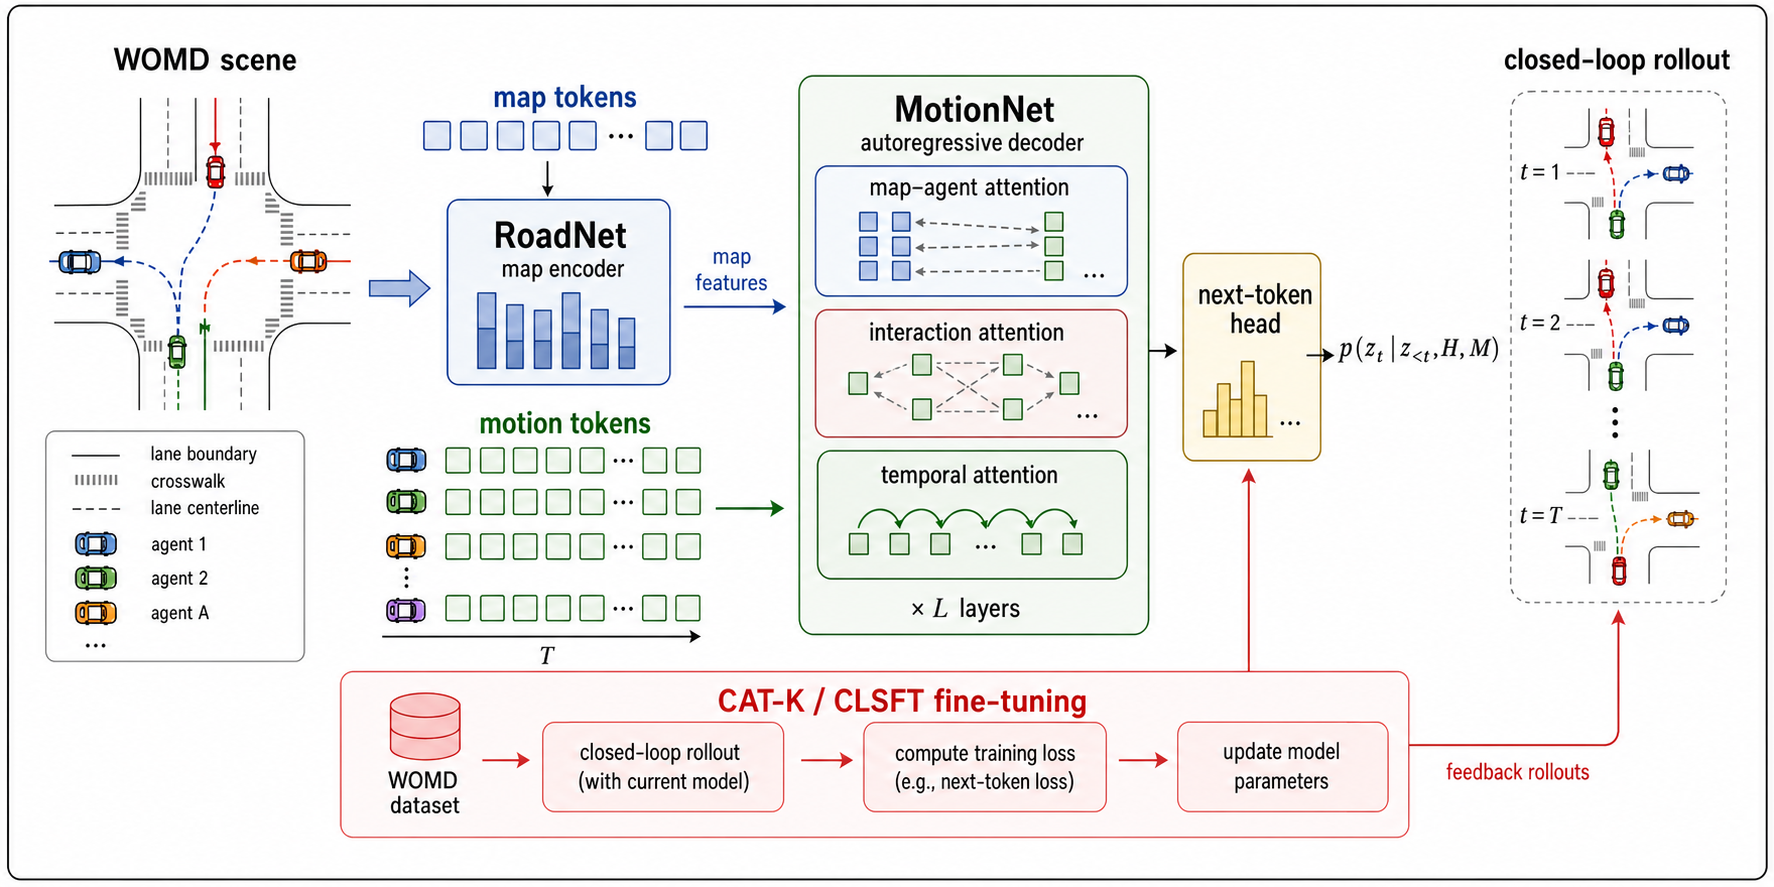
\includegraphics[width=\linewidth,height=0.66\textheight,keepaspectratio]{../assets/figures/method/smart_catk_ntp_pipeline_imagegen_20260425.png}
    \end{column}
  \end{columns}
\end{frame}

\begin{frame}{Waymax-Backed Diagnostic Phases}
  \begin{columns}[T,totalwidth=\textwidth]
    \begin{column}{0.24\textwidth}
      \phasebox{Phase 1}{Branch execution}{Run normal, forced, and placebo branches from the same Waymax simulator state.}
    \end{column}
    \begin{column}{0.24\textwidth}
      \phasebox{Phase 2}{Structural scoring}{Measure gap, TTC, response delay, collision, offroad, and placebo deviation.}
    \end{column}
    \begin{column}{0.24\textwidth}
      \phasebox{Phase 3}{Critic validation}{Train a small critic only if branch labels survive held-out and placebo gates.}
    \end{column}
    \begin{column}{0.24\textwidth}
      \phasebox{Phase 4}{Conservative adaptation}{Fine-tune only with KL anchoring, replay, and WOSAC realism budgets.}
    \end{column}
  \end{columns}
  \vspace{0.45cm}
  \begin{center}
    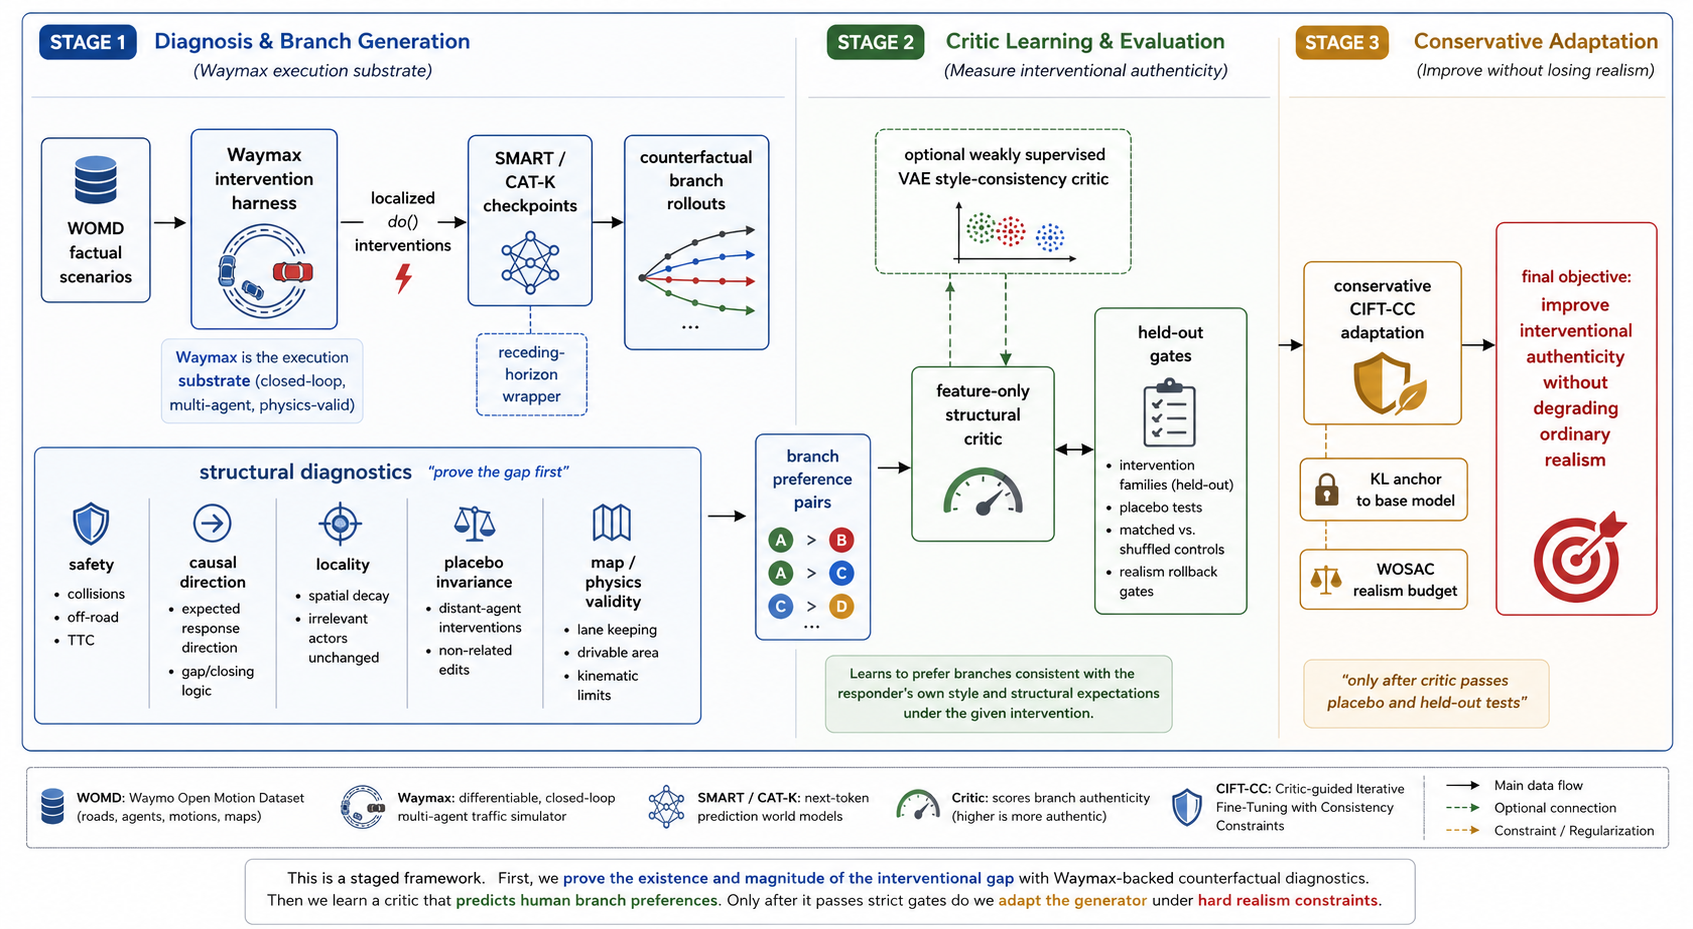
\includegraphics[width=0.82\linewidth,height=0.34\textheight,keepaspectratio]{../assets/figures/method/traffic_authenticity_waymax_ciftcc_pipeline_imagegen_20260427.png}
  \end{center}
\end{frame}

\begin{frame}{Proposed Algorithms}
  \begin{columns}[T,totalwidth=\textwidth]
    \begin{column}{0.48\textwidth}
      \textbf{Algorithm 1: diagnostic evaluation}
      \begin{enumerate}\tightitem
        \item Load WOMD scenario and initialize Waymax state.
        \item Run normal rollout with policy $\pi$.
        \item Construct a valid forced branch for each intervention family.
        \item Run forced and placebo branches from the same state.
        \item Compute gap, TTC, speed response, collision, offroad, and placebo features.
        \item Aggregate TIA/CIRS by model, scenario, family, and branch pair.
      \end{enumerate}
    \end{column}
    \begin{column}{0.48\textwidth}
      \textbf{Algorithm 2: critic-gated adaptation}
      \begin{enumerate}\tightitem
        \item Build branch preference pairs from validated diagnostics.
        \item Train small structural critics first.
        \item Reject critics that fail held-out or placebo tests.
        \item Optionally add style-consistency after structural gates pass.
        \item Fine-tune only with KL, replay, and realism budgets.
        \item Roll back any checkpoint that improves TIA while hurting WOSAC realism.
      \end{enumerate}
    \end{column}
  \end{columns}
\end{frame}

\begin{frame}{Qualitative Rollout Triptych}
  \begin{columns}[T,totalwidth=\textwidth]
    \begin{column}{0.32\textwidth}
      \centering\textbf{Ground Truth}\par\vspace{0.12cm}
      \image[width=0.30,aspectratio=16/9,fit=contain,draw] {\detokenize{../assets/videos/lead_braking_case_01/ground_truth.gif}}
    \end{column}
    \begin{column}{0.32\textwidth}
      \centering\textbf{SMART-BC}\par\vspace{0.12cm}
      \image[width=0.30,aspectratio=16/9,fit=contain,draw] {\detokenize{../assets/videos/lead_braking_case_01/smart_bc.gif}}
    \end{column}
    \begin{column}{0.32\textwidth}
      \centering\textbf{SMART-CLSFT}\par\vspace{0.12cm}
      \image[width=0.30,aspectratio=16/9,fit=contain,draw] {\detokenize{../assets/videos/lead_braking_case_01/smart_clsft.gif}}
    \end{column}
  \end{columns}
  \vspace{0.35cm}
  \small The Reveal export overlays browser-native animated media on top of the Beamer-authored PDF slide. This is the main reason to use \texttt{beamer-reveal} instead of plain PDF Beamer.
\end{frame}

\begin{frame}{Build Decision}
  \claimbox{Recommendation}{Use Beamer + LuaLaTeX + beamer-reveal for the thesis-review deck if precise layout control matters more than rapid markdown editing. Keep Quarto only for static research-note websites or as a landing page, not as the slide authoring layer.}
  \vspace{0.35cm}
  \begin{itemize}\tightitem
    \item Beamer gives hard slide boundaries: if content overflows, it is visible during compilation and fixable at source level.
    \item TikZ, equations, tables, and block geometry are fully controllable.
    \item Reveal export keeps browser presentation, GIF/video overlays, speaker notes, and keyboard navigation.
    \item The cost is a heavier build pipeline and less markdown convenience.
  \end{itemize}
\end{frame}

\end{document}
